\documentclass[1p]{elsarticle_modified}
%\bibliographystyle{elsarticle-num}

%\usepackage[colorlinks]{hyperref}
%\usepackage{abbrmath_seonhwa} %\Abb, \Ascr, \Acal ,\Abf, \Afrak
\usepackage{amsfonts}
\usepackage{amssymb}
\usepackage{amsmath}
\usepackage{amsthm}
\usepackage{scalefnt}
\usepackage{amsbsy}
\usepackage{kotex}
\usepackage{caption}
\usepackage{subfig}
\usepackage{color}
\usepackage{graphicx}
\usepackage{xcolor} %% white, black, red, green, blue, cyan, magenta, yellow
\usepackage{float}
\usepackage{setspace}
\usepackage{hyperref}

\usepackage{tikz}
\usetikzlibrary{arrows}

\usepackage{multirow}
\usepackage{array} % fixed length table
\usepackage{hhline}

%%%%%%%%%%%%%%%%%%%%%
\makeatletter
\renewcommand*\env@matrix[1][\arraystretch]{%
	\edef\arraystretch{#1}%
	\hskip -\arraycolsep
	\let\@ifnextchar\new@ifnextchar
	\array{*\c@MaxMatrixCols c}}
\makeatother %https://tex.stackexchange.com/questions/14071/how-can-i-increase-the-line-spacing-in-a-matrix
%%%%%%%%%%%%%%%

\usepackage[normalem]{ulem}

\newcommand{\msout}[1]{\ifmmode\text{\sout{\ensuremath{#1}}}\else\sout{#1}\fi}
%SOURCE: \msout is \stkout macro in https://tex.stackexchange.com/questions/20609/strikeout-in-math-mode

\newcommand{\cancel}[1]{
	\ifmmode
	{\color{red}\msout{#1}}
	\else
	{\color{red}\sout{#1}}
	\fi
}

\newcommand{\add}[1]{
	{\color{blue}\uwave{#1}}
}

\newcommand{\replace}[2]{
	\ifmmode
	{\color{red}\msout{#1}}{\color{blue}\uwave{#2}}
	\else
	{\color{red}\sout{#1}}{\color{blue}\uwave{#2}}
	\fi
}

\newcommand{\Sol}{\mathcal{S}} %segment
\newcommand{\D}{D} %diagram
\newcommand{\A}{\mathcal{A}} %arc


%%%%%%%%%%%%%%%%%%%%%%%%%%%%%5 test

\def\sl{\operatorname{\textup{SL}}(2,\Cbb)}
\def\psl{\operatorname{\textup{PSL}}(2,\Cbb)}
\def\quan{\mkern 1mu \triangleright \mkern 1mu}

\theoremstyle{definition}
\newtheorem{thm}{Theorem}[section]
\newtheorem{prop}[thm]{Proposition}
\newtheorem{lem}[thm]{Lemma}
\newtheorem{ques}[thm]{Question}
\newtheorem{cor}[thm]{Corollary}
\newtheorem{defn}[thm]{Definition}
\newtheorem{exam}[thm]{Example}
\newtheorem{rmk}[thm]{Remark}
\newtheorem{alg}[thm]{Algorithm}

\newcommand{\I}{\sqrt{-1}}
\begin{document}

%\begin{frontmatter}
%
%\title{Boundary parabolic representations of knots up to 8 crossings}
%
%%% Group authors per affiliation:
%\author{Yunhi Cho} 
%\address{Department of Mathematics, University of Seoul, Seoul, Korea}
%\ead{yhcho@uos.ac.kr}
%
%
%\author{Seonhwa Kim} %\fnref{s_kim}}
%\address{Center for Geometry and Physics, Institute for Basic Science, Pohang, 37673, Korea}
%\ead{ryeona17@ibs.re.kr}
%
%\author{Hyuk Kim}
%\address{Department of Mathematical Sciences, Seoul National University, Seoul 08826, Korea}
%\ead{hyukkim@snu.ac.kr}
%
%\author{Seokbeom Yoon}
%\address{Department of Mathematical Sciences, Seoul National University, Seoul, 08826,  Korea}
%\ead{sbyoon15@snu.ac.kr}
%
%\begin{abstract}
%We find all boundary parabolic representation of knots up to 8 crossings.
%
%\end{abstract}
%\begin{keyword}
%    \MSC[2010] 57M25 
%\end{keyword}
%
%\end{frontmatter}

%\linenumbers
%\tableofcontents
%
\newcommand\colored[1]{\textcolor{white}{\rule[-0.35ex]{0.8em}{1.4ex}}\kern-0.8em\color{red} #1}%
%\newcommand\colored[1]{\textcolor{white}{ #1}\kern-2.17ex	\textcolor{white}{ #1}\kern-1.81ex	\textcolor{white}{ #1}\kern-2.15ex\color{red}#1	}

{\Large $\underline{12a_{0512}~(K12a_{0512})}$}

\setlength{\tabcolsep}{10pt}
\renewcommand{\arraystretch}{1.6}
\vspace{1cm}\begin{tabular}{m{100pt}>{\centering\arraybackslash}m{274pt}}
\multirow{5}{120pt}{
	\centering
	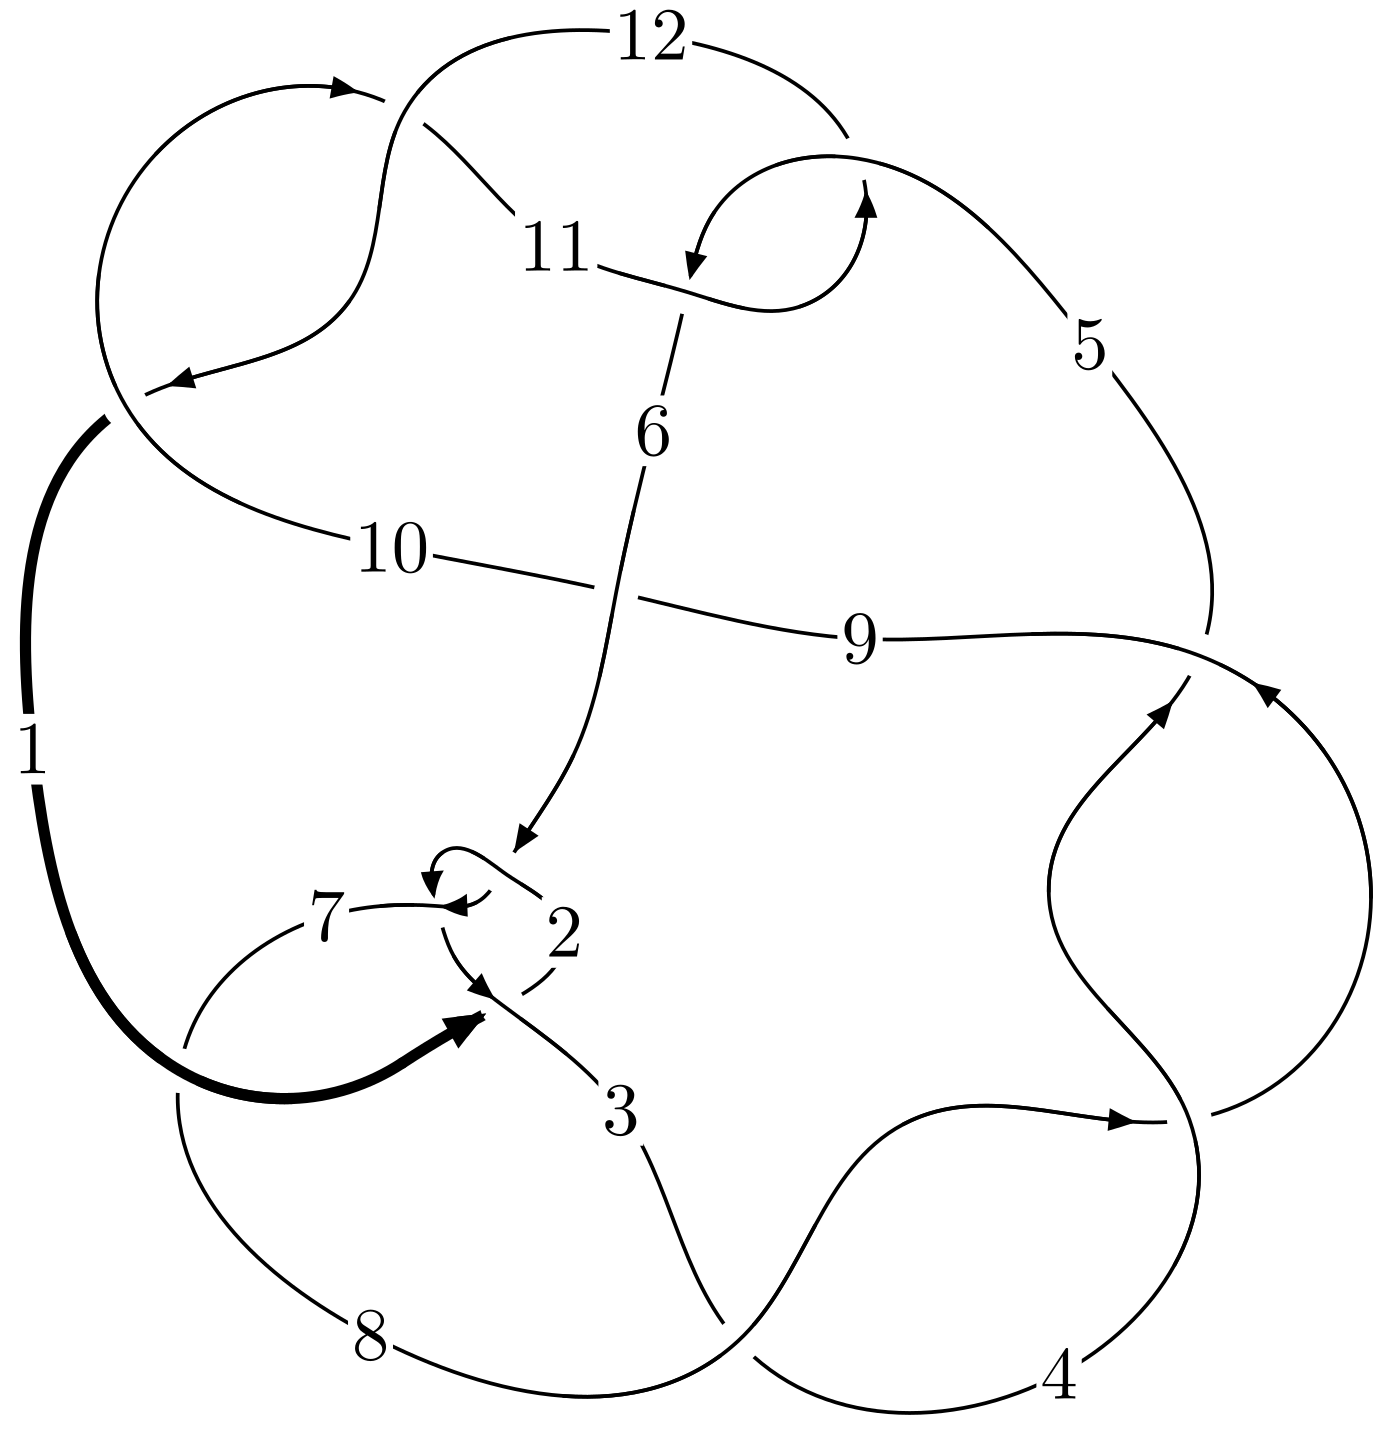
\includegraphics[width=112pt]{../../../GIT/diagram.site/Diagrams/png/1313_12a_0512.png}\\
\ \ \ A knot diagram\footnotemark}&
\allowdisplaybreaks
\textbf{Linearized knot diagam} \\
\cline{2-2}
 &
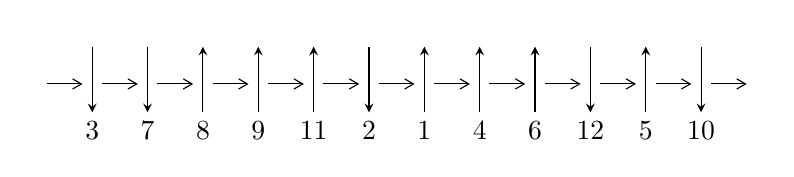
\begin{tikzpicture}[x=20pt, y=17pt]
	% nodes
	\node (C0) at (0, 0) {};
	\node (C1) at (1, 0) {};
	\node (C1U) at (1, +1) {};
	\node (C1D) at (1, -1) {3};

	\node (C2) at (2, 0) {};
	\node (C2U) at (2, +1) {};
	\node (C2D) at (2, -1) {7};

	\node (C3) at (3, 0) {};
	\node (C3U) at (3, +1) {};
	\node (C3D) at (3, -1) {8};

	\node (C4) at (4, 0) {};
	\node (C4U) at (4, +1) {};
	\node (C4D) at (4, -1) {9};

	\node (C5) at (5, 0) {};
	\node (C5U) at (5, +1) {};
	\node (C5D) at (5, -1) {11};

	\node (C6) at (6, 0) {};
	\node (C6U) at (6, +1) {};
	\node (C6D) at (6, -1) {2};

	\node (C7) at (7, 0) {};
	\node (C7U) at (7, +1) {};
	\node (C7D) at (7, -1) {1};

	\node (C8) at (8, 0) {};
	\node (C8U) at (8, +1) {};
	\node (C8D) at (8, -1) {4};

	\node (C9) at (9, 0) {};
	\node (C9U) at (9, +1) {};
	\node (C9D) at (9, -1) {6};

	\node (C10) at (10, 0) {};
	\node (C10U) at (10, +1) {};
	\node (C10D) at (10, -1) {12};

	\node (C11) at (11, 0) {};
	\node (C11U) at (11, +1) {};
	\node (C11D) at (11, -1) {5};

	\node (C12) at (12, 0) {};
	\node (C12U) at (12, +1) {};
	\node (C12D) at (12, -1) {10};
	\node (C13) at (13, 0) {};

	% arrows
	\draw[->,>={angle 60}]
	(C0) edge (C1) (C1) edge (C2) (C2) edge (C3) (C3) edge (C4) (C4) edge (C5) (C5) edge (C6) (C6) edge (C7) (C7) edge (C8) (C8) edge (C9) (C9) edge (C10) (C10) edge (C11) (C11) edge (C12) (C12) edge (C13) ;	\draw[->,>=stealth]
	(C1U) edge (C1D) (C2U) edge (C2D) (C3D) edge (C3U) (C4D) edge (C4U) (C5D) edge (C5U) (C6U) edge (C6D) (C7D) edge (C7U) (C8D) edge (C8U) (C9D) edge (C9U) (C10U) edge (C10D) (C11D) edge (C11U) (C12U) edge (C12D) ;
	\end{tikzpicture} \\
\hhline{~~} \\& 
\textbf{Solving Sequence} \\ \cline{2-2} 
 &
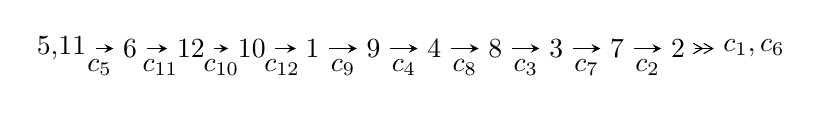
\begin{tikzpicture}[x=22pt, y=7pt]
	% node
	\node (A0) at (-1/8, 0) {5,11};
	\node (A1) at (1, 0) {6};
	\node (A2) at (2, 0) {12};
	\node (A3) at (3, 0) {10};
	\node (A4) at (4, 0) {1};
	\node (A5) at (5, 0) {9};
	\node (A6) at (6, 0) {4};
	\node (A7) at (7, 0) {8};
	\node (A8) at (8, 0) {3};
	\node (A9) at (9, 0) {7};
	\node (A10) at (10, 0) {2};
	\node (C1) at (1/2, -1) {$c_{5}$};
	\node (C2) at (3/2, -1) {$c_{11}$};
	\node (C3) at (5/2, -1) {$c_{10}$};
	\node (C4) at (7/2, -1) {$c_{12}$};
	\node (C5) at (9/2, -1) {$c_{9}$};
	\node (C6) at (11/2, -1) {$c_{4}$};
	\node (C7) at (13/2, -1) {$c_{8}$};
	\node (C8) at (15/2, -1) {$c_{3}$};
	\node (C9) at (17/2, -1) {$c_{7}$};
	\node (C10) at (19/2, -1) {$c_{2}$};
	\node (A11) at (45/4, 0) {$c_{1},c_{6}$};

	% edge
	\draw[->,>=stealth]	
	(A0) edge (A1) (A1) edge (A2) (A2) edge (A3) (A3) edge (A4) (A4) edge (A5) (A5) edge (A6) (A6) edge (A7) (A7) edge (A8) (A8) edge (A9) (A9) edge (A10) ;
	\draw[->>,>={angle 60}]	
	(A10) edge (A11);
\end{tikzpicture} \\ 

\end{tabular} \\

\footnotetext{
The image of knot diagram is generated by the software ``\textbf{Draw programme}" developed by Andrew Bartholomew(\url{http://www.layer8.co.uk/maths/draw/index.htm\#Running-draw}), where we modified some parts for our purpose(\url{https://github.com/CATsTAILs/LinksPainter}).
}\phantom \\ \newline 
\centering \textbf{Ideals for irreducible components\footnotemark of $X_{\text{par}}$} 
 
\begin{align*}
I^u_{1}&=\langle 
u^{75}+u^{74}+\cdots+u^2-1\rangle \\
\\
\end{align*}
\raggedright * 1 irreducible components of $\dim_{\mathbb{C}}=0$, with total 75 representations.\\
\footnotetext{All coefficients of polynomials are rational numbers. But the coefficients are sometimes approximated in decimal forms when there is not enough margin.}
\newpage
\renewcommand{\arraystretch}{1}
\centering \section*{I. $I^u_{1}= \langle u^{75}+u^{74}+\cdots+u^2-1 \rangle$}
\flushleft \textbf{(i) Arc colorings}\\
\begin{tabular}{m{7pt} m{180pt} m{7pt} m{180pt} }
\flushright $a_{5}=$&$\begin{pmatrix}1\\0\end{pmatrix}$ \\
\flushright $a_{11}=$&$\begin{pmatrix}0\\u\end{pmatrix}$ \\
\flushright $a_{6}=$&$\begin{pmatrix}1\\- u^2\end{pmatrix}$ \\
\flushright $a_{12}=$&$\begin{pmatrix}u\\u\end{pmatrix}$ \\
\flushright $a_{10}=$&$\begin{pmatrix}u^3\\u^3+u\end{pmatrix}$ \\
\flushright $a_{1}=$&$\begin{pmatrix}u^5+u\\u^5+u^3+u\end{pmatrix}$ \\
\flushright $a_{9}=$&$\begin{pmatrix}- u^5- u\\u^7+u^5+2 u^3+u\end{pmatrix}$ \\
\flushright $a_{4}=$&$\begin{pmatrix}- u^{12}- u^{10}-3 u^8-2 u^6-2 u^4- u^2+1\\u^{14}+2 u^{12}+5 u^{10}+6 u^8+6 u^6+4 u^4+u^2\end{pmatrix}$ \\
\flushright $a_{8}=$&$\begin{pmatrix}u^{19}+2 u^{17}+6 u^{15}+8 u^{13}+11 u^{11}+10 u^9+6 u^7+2 u^5- u^3-2 u\\- u^{21}-3 u^{19}+\cdots+u^3+u\end{pmatrix}$ \\
\flushright $a_{3}=$&$\begin{pmatrix}u^{26}+3 u^{24}+\cdots-3 u^2+1\\- u^{28}-4 u^{26}+\cdots+7 u^4+2 u^2\end{pmatrix}$ \\
\flushright $a_{7}=$&$\begin{pmatrix}u^{31}+4 u^{29}+\cdots-4 u^3-2 u\\u^{31}+5 u^{29}+\cdots-2 u^3+u\end{pmatrix}$ \\
\flushright $a_{2}=$&$\begin{pmatrix}- u^{59}-8 u^{57}+\cdots+12 u^5+7 u^3\\u^{61}+9 u^{59}+\cdots- u^3+u\end{pmatrix}$\\&\end{tabular}
\flushleft \textbf{(ii) Obstruction class $= -1$}\\~\\
\flushleft \textbf{(iii) Cusp Shapes $= 4 u^{73}+4 u^{72}+\cdots+8 u+2$}\\~\\
\newpage\renewcommand{\arraystretch}{1}
\flushleft \textbf{(iv) u-Polynomials at the component}\newline \\
\begin{tabular}{m{50pt}|m{274pt}}
Crossings & \hspace{64pt}u-Polynomials at each crossing \\
\hline $$\begin{aligned}c_{1}\end{aligned}$$&$\begin{aligned}
&u^{75}+33 u^{74}+\cdots+2 u+1
\end{aligned}$\\
\hline $$\begin{aligned}c_{2},c_{6}\end{aligned}$$&$\begin{aligned}
&u^{75}- u^{74}+\cdots+u^2-1
\end{aligned}$\\
\hline $$\begin{aligned}c_{3},c_{4},c_{8}\end{aligned}$$&$\begin{aligned}
&u^{75}+u^{74}+\cdots-110 u-25
\end{aligned}$\\
\hline $$\begin{aligned}c_{5},c_{11}\end{aligned}$$&$\begin{aligned}
&u^{75}+u^{74}+\cdots+u^2-1
\end{aligned}$\\
\hline $$\begin{aligned}c_{7}\end{aligned}$$&$\begin{aligned}
&u^{75}-3 u^{74}+\cdots-8 u+3
\end{aligned}$\\
\hline $$\begin{aligned}c_{9}\end{aligned}$$&$\begin{aligned}
&u^{75}-5 u^{74}+\cdots+21044 u-3477
\end{aligned}$\\
\hline $$\begin{aligned}c_{10},c_{12}\end{aligned}$$&$\begin{aligned}
&u^{75}+23 u^{74}+\cdots+2 u-1
\end{aligned}$\\
\hline
\end{tabular}\\~\\
\newpage\renewcommand{\arraystretch}{1}
\flushleft \textbf{(v) Riley Polynomials at the component}\newline \\
\begin{tabular}{m{50pt}|m{274pt}}
Crossings & \hspace{64pt}Riley Polynomials at each crossing \\
\hline $$\begin{aligned}c_{1}\end{aligned}$$&$\begin{aligned}
&y^{75}+19 y^{74}+\cdots-10 y-1
\end{aligned}$\\
\hline $$\begin{aligned}c_{2},c_{6}\end{aligned}$$&$\begin{aligned}
&y^{75}-33 y^{74}+\cdots+2 y-1
\end{aligned}$\\
\hline $$\begin{aligned}c_{3},c_{4},c_{8}\end{aligned}$$&$\begin{aligned}
&y^{75}-81 y^{74}+\cdots+28950 y-625
\end{aligned}$\\
\hline $$\begin{aligned}c_{5},c_{11}\end{aligned}$$&$\begin{aligned}
&y^{75}+23 y^{74}+\cdots+2 y-1
\end{aligned}$\\
\hline $$\begin{aligned}c_{7}\end{aligned}$$&$\begin{aligned}
&y^{75}-5 y^{74}+\cdots+562 y-9
\end{aligned}$\\
\hline $$\begin{aligned}c_{9}\end{aligned}$$&$\begin{aligned}
&y^{75}-29 y^{74}+\cdots+182318326 y-12089529
\end{aligned}$\\
\hline $$\begin{aligned}c_{10},c_{12}\end{aligned}$$&$\begin{aligned}
&y^{75}+59 y^{74}+\cdots+22 y-1
\end{aligned}$\\
\hline
\end{tabular}\\~\\
\newpage\flushleft \textbf{(vi) Complex Volumes and Cusp Shapes}
$$\begin{array}{c|c|c}  
\text{Solutions to }I^u_{1}& \I (\text{vol} + \sqrt{-1}CS) & \text{Cusp shape}\\
 \hline 
\begin{aligned}
u &= \phantom{-}0.682193 + 0.732664 I\end{aligned}
 & -0.302285 + 0.979820 I & \phantom{-0.000000 } 0 \\ \hline\begin{aligned}
u &= \phantom{-}0.682193 - 0.732664 I\end{aligned}
 & -0.302285 - 0.979820 I & \phantom{-0.000000 } 0 \\ \hline\begin{aligned}
u &= -0.101406 + 0.992248 I\end{aligned}
 & -4.21065 - 6.07424 I & -4.70014 + 8.18701 I \\ \hline\begin{aligned}
u &= -0.101406 - 0.992248 I\end{aligned}
 & -4.21065 + 6.07424 I & -4.70014 - 8.18701 I \\ \hline\begin{aligned}
u &= -0.044728 + 0.980361 I\end{aligned}
 & -5.29212 + 0.73505 I & -7.97312 + 0. I\phantom{ +0.000000I} \\ \hline\begin{aligned}
u &= -0.044728 - 0.980361 I\end{aligned}
 & -5.29212 - 0.73505 I & -7.97312 + 0. I\phantom{ +0.000000I} \\ \hline\begin{aligned}
u &= \phantom{-}0.231455 + 1.000170 I\end{aligned}
 & -0.58521 + 2.91346 I & \phantom{-0.000000 } 0 \\ \hline\begin{aligned}
u &= \phantom{-}0.231455 - 1.000170 I\end{aligned}
 & -0.58521 - 2.91346 I & \phantom{-0.000000 } 0 \\ \hline\begin{aligned}
u &= \phantom{-}0.748094 + 0.708104 I\end{aligned}
 & \phantom{-}1.49916 - 5.73552 I & \phantom{-0.000000 } 0 \\ \hline\begin{aligned}
u &= \phantom{-}0.748094 - 0.708104 I\end{aligned}
 & \phantom{-}1.49916 + 5.73552 I & \phantom{-0.000000 } 0 \\ \hline\begin{aligned}
u &= \phantom{-}0.277622 + 1.006300 I\end{aligned}
 & \phantom{-}3.26637 - 3.71880 I & \phantom{-0.000000 } 0 \\ \hline\begin{aligned}
u &= \phantom{-}0.277622 - 1.006300 I\end{aligned}
 & \phantom{-}3.26637 + 3.71880 I & \phantom{-0.000000 } 0 \\ \hline\begin{aligned}
u &= \phantom{-}0.099815 + 0.950570 I\end{aligned}
 & -2.03163 + 1.90280 I & -1.00812 - 4.53925 I \\ \hline\begin{aligned}
u &= \phantom{-}0.099815 - 0.950570 I\end{aligned}
 & -2.03163 - 1.90280 I & -1.00812 + 4.53925 I \\ \hline\begin{aligned}
u &= -0.265572 + 1.012460 I\end{aligned}
 & \phantom{-}4.96981 - 1.56282 I & \phantom{-0.000000 } 0 \\ \hline\begin{aligned}
u &= -0.265572 - 1.012460 I\end{aligned}
 & \phantom{-}4.96981 + 1.56282 I & \phantom{-0.000000 } 0 \\ \hline\begin{aligned}
u &= -0.586679 + 0.867149 I\end{aligned}
 & -1.77126 + 1.03509 I & \phantom{-0.000000 } 0 \\ \hline\begin{aligned}
u &= -0.586679 - 0.867149 I\end{aligned}
 & -1.77126 - 1.03509 I & \phantom{-0.000000 } 0 \\ \hline\begin{aligned}
u &= -0.746947 + 0.736867 I\end{aligned}
 & \phantom{-}3.53722 + 1.18244 I & \phantom{-0.000000 } 0 \\ \hline\begin{aligned}
u &= -0.746947 - 0.736867 I\end{aligned}
 & \phantom{-}3.53722 - 1.18244 I & \phantom{-0.000000 } 0 \\ \hline\begin{aligned}
u &= -0.242468 + 1.028110 I\end{aligned}
 & \phantom{-}4.79959 - 4.64962 I & \phantom{-0.000000 } 0 \\ \hline\begin{aligned}
u &= -0.242468 - 1.028110 I\end{aligned}
 & \phantom{-}4.79959 + 4.64962 I & \phantom{-0.000000 } 0 \\ \hline\begin{aligned}
u &= \phantom{-}0.234800 + 1.034640 I\end{aligned}
 & \phantom{-}2.95579 + 9.94979 I & \phantom{-0.000000 } 0 \\ \hline\begin{aligned}
u &= \phantom{-}0.234800 - 1.034640 I\end{aligned}
 & \phantom{-}2.95579 - 9.94979 I & \phantom{-0.000000 } 0 \\ \hline\begin{aligned}
u &= \phantom{-}0.647448 + 0.875979 I\end{aligned}
 & \phantom{-}0.73242 + 2.51663 I & \phantom{-0.000000 } 0 \\ \hline\begin{aligned}
u &= \phantom{-}0.647448 - 0.875979 I\end{aligned}
 & \phantom{-}0.73242 - 2.51663 I & \phantom{-0.000000 } 0 \\ \hline\begin{aligned}
u &= -0.758459 + 0.794993 I\end{aligned}
 & \phantom{-}4.55012 - 0.14668 I & \phantom{-0.000000 } 0 \\ \hline\begin{aligned}
u &= -0.758459 - 0.794993 I\end{aligned}
 & \phantom{-}4.55012 + 0.14668 I & \phantom{-0.000000 } 0 \\ \hline\begin{aligned}
u &= -0.628084 + 0.921139 I\end{aligned}
 & -2.04419 - 5.77241 I & \phantom{-0.000000 } 0 \\ \hline\begin{aligned}
u &= -0.628084 - 0.921139 I\end{aligned}
 & -2.04419 + 5.77241 I & \phantom{-0.000000 } 0\\
 \hline 
 \end{array}$$\newpage$$\begin{array}{c|c|c}  
\text{Solutions to }I^u_{1}& \I (\text{vol} + \sqrt{-1}CS) & \text{Cusp shape}\\
 \hline 
\begin{aligned}
u &= -0.835257 + 0.742674 I\end{aligned}
 & \phantom{-}6.35107 + 2.04623 I & \phantom{-0.000000 } 0 \\ \hline\begin{aligned}
u &= -0.835257 - 0.742674 I\end{aligned}
 & \phantom{-}6.35107 - 2.04623 I & \phantom{-0.000000 } 0 \\ \hline\begin{aligned}
u &= \phantom{-}0.758172 + 0.825776 I\end{aligned}
 & \phantom{-}3.58561 + 4.71802 I & \phantom{-0.000000 } 0 \\ \hline\begin{aligned}
u &= \phantom{-}0.758172 - 0.825776 I\end{aligned}
 & \phantom{-}3.58561 - 4.71802 I & \phantom{-0.000000 } 0 \\ \hline\begin{aligned}
u &= -0.847393 + 0.734484 I\end{aligned}
 & \phantom{-}10.08040 + 9.29957 I & \phantom{-0.000000 } 0 \\ \hline\begin{aligned}
u &= -0.847393 - 0.734484 I\end{aligned}
 & \phantom{-}10.08040 - 9.29957 I & \phantom{-0.000000 } 0 \\ \hline\begin{aligned}
u &= \phantom{-}0.846821 + 0.739280 I\end{aligned}
 & \phantom{-}11.94220 - 3.91143 I & \phantom{-0.000000 } 0 \\ \hline\begin{aligned}
u &= \phantom{-}0.846821 - 0.739280 I\end{aligned}
 & \phantom{-}11.94220 + 3.91143 I & \phantom{-0.000000 } 0 \\ \hline\begin{aligned}
u &= \phantom{-}0.845301 + 0.751762 I\end{aligned}
 & \phantom{-}12.17070 - 0.58717 I & \phantom{-0.000000 } 0 \\ \hline\begin{aligned}
u &= \phantom{-}0.845301 - 0.751762 I\end{aligned}
 & \phantom{-}12.17070 + 0.58717 I & \phantom{-0.000000 } 0 \\ \hline\begin{aligned}
u &= -0.844440 + 0.757264 I\end{aligned}
 & \phantom{-}10.49740 - 4.80557 I & \phantom{-0.000000 } 0 \\ \hline\begin{aligned}
u &= -0.844440 - 0.757264 I\end{aligned}
 & \phantom{-}10.49740 + 4.80557 I & \phantom{-0.000000 } 0 \\ \hline\begin{aligned}
u &= \phantom{-}0.738716 + 0.913060 I\end{aligned}
 & \phantom{-}3.31838 + 0.95336 I & \phantom{-0.000000 } 0 \\ \hline\begin{aligned}
u &= \phantom{-}0.738716 - 0.913060 I\end{aligned}
 & \phantom{-}3.31838 - 0.95336 I & \phantom{-0.000000 } 0 \\ \hline\begin{aligned}
u &= \phantom{-}0.682106 + 0.959266 I\end{aligned}
 & -0.98202 + 4.31584 I & \phantom{-0.000000 } 0 \\ \hline\begin{aligned}
u &= \phantom{-}0.682106 - 0.959266 I\end{aligned}
 & -0.98202 - 4.31584 I & \phantom{-0.000000 } 0 \\ \hline\begin{aligned}
u &= -0.731393 + 0.936292 I\end{aligned}
 & \phantom{-}4.12042 - 5.50383 I & \phantom{-0.000000 } 0 \\ \hline\begin{aligned}
u &= -0.731393 - 0.936292 I\end{aligned}
 & \phantom{-}4.12042 + 5.50383 I & \phantom{-0.000000 } 0 \\ \hline\begin{aligned}
u &= \phantom{-}0.158699 + 0.795794 I\end{aligned}
 & -0.93723 + 1.74811 I & \phantom{-}1.58765 - 5.17968 I \\ \hline\begin{aligned}
u &= \phantom{-}0.158699 - 0.795794 I\end{aligned}
 & -0.93723 - 1.74811 I & \phantom{-}1.58765 + 5.17968 I \\ \hline\begin{aligned}
u &= -0.709189 + 0.967062 I\end{aligned}
 & \phantom{-}2.84545 - 6.72964 I & \phantom{-0.000000 } 0 \\ \hline\begin{aligned}
u &= -0.709189 - 0.967062 I\end{aligned}
 & \phantom{-}2.84545 + 6.72964 I & \phantom{-0.000000 } 0 \\ \hline\begin{aligned}
u &= \phantom{-}0.702838 + 0.980436 I\end{aligned}
 & \phantom{-}0.68737 + 11.26350 I & \phantom{-0.000000 } 0 \\ \hline\begin{aligned}
u &= \phantom{-}0.702838 - 0.980436 I\end{aligned}
 & \phantom{-}0.68737 - 11.26350 I & \phantom{-0.000000 } 0 \\ \hline\begin{aligned}
u &= -0.753756 + 0.996096 I\end{aligned}
 & \phantom{-}5.57098 - 7.98818 I & \phantom{-0.000000 } 0 \\ \hline\begin{aligned}
u &= -0.753756 - 0.996096 I\end{aligned}
 & \phantom{-}5.57098 + 7.98818 I & \phantom{-0.000000 } 0 \\ \hline\begin{aligned}
u &= -0.765394 + 0.991927 I\end{aligned}
 & \phantom{-}9.77291 - 1.20159 I & \phantom{-0.000000 } 0 \\ \hline\begin{aligned}
u &= -0.765394 - 0.991927 I\end{aligned}
 & \phantom{-}9.77291 + 1.20159 I & \phantom{-0.000000 } 0 \\ \hline\begin{aligned}
u &= \phantom{-}0.763313 + 0.995423 I\end{aligned}
 & \phantom{-}11.41870 + 6.58981 I & \phantom{-0.000000 } 0 \\ \hline\begin{aligned}
u &= \phantom{-}0.763313 - 0.995423 I\end{aligned}
 & \phantom{-}11.41870 - 6.58981 I & \phantom{-0.000000 } 0\\
 \hline 
 \end{array}$$\newpage$$\begin{array}{c|c|c}  
\text{Solutions to }I^u_{1}& \I (\text{vol} + \sqrt{-1}CS) & \text{Cusp shape}\\
 \hline 
\begin{aligned}
u &= \phantom{-}0.758437 + 1.002770 I\end{aligned}
 & \phantom{-}11.1297 + 9.9017 I & \phantom{-0.000000 } 0 \\ \hline\begin{aligned}
u &= \phantom{-}0.758437 - 1.002770 I\end{aligned}
 & \phantom{-}11.1297 - 9.9017 I & \phantom{-0.000000 } 0 \\ \hline\begin{aligned}
u &= -0.756608 + 1.005470 I\end{aligned}
 & \phantom{-}9.2451 - 15.2850 I & \phantom{-0.000000 } 0 \\ \hline\begin{aligned}
u &= -0.756608 - 1.005470 I\end{aligned}
 & \phantom{-}9.2451 + 15.2850 I & \phantom{-0.000000 } 0 \\ \hline\begin{aligned}
u &= \phantom{-}0.686093 + 0.028981 I\end{aligned}
 & \phantom{-}6.40339 + 6.93089 I & \phantom{-}7.58937 - 5.03714 I \\ \hline\begin{aligned}
u &= \phantom{-}0.686093 - 0.028981 I\end{aligned}
 & \phantom{-}6.40339 - 6.93089 I & \phantom{-}7.58937 + 5.03714 I \\ \hline\begin{aligned}
u &= -0.685171 + 0.015873 I\end{aligned}
 & \phantom{-}8.17683 - 1.59594 I & \phantom{-}10.20433 + 0.32100 I \\ \hline\begin{aligned}
u &= -0.685171 - 0.015873 I\end{aligned}
 & \phantom{-}8.17683 + 1.59594 I & \phantom{-}10.20433 - 0.32100 I \\ \hline\begin{aligned}
u &= \phantom{-}0.652464\phantom{ +0.000000I}\end{aligned}
 & \phantom{-}2.61478\phantom{ +0.000000I} & \phantom{-}4.37850\phantom{ +0.000000I} \\ \hline\begin{aligned}
u &= -0.334129 + 0.411688 I\end{aligned}
 & -1.50019 + 1.55713 I & \phantom{-}0.650340 - 0.272682 I \\ \hline\begin{aligned}
u &= -0.334129 - 0.411688 I\end{aligned}
 & -1.50019 - 1.55713 I & \phantom{-}0.650340 + 0.272682 I \\ \hline\begin{aligned}
u &= -0.480157 + 0.207491 I\end{aligned}
 & -0.60976 - 4.42214 I & \phantom{-}4.50486 + 7.49216 I \\ \hline\begin{aligned}
u &= -0.480157 - 0.207491 I\end{aligned}
 & -0.60976 + 4.42214 I & \phantom{-}4.50486 - 7.49216 I \\ \hline\begin{aligned}
u &= \phantom{-}0.429074 + 0.095570 I\end{aligned}
 & \phantom{-}1.039040 + 0.315096 I & \phantom{-}9.75730 - 1.79361 I \\ \hline\begin{aligned}
u &= \phantom{-}0.429074 - 0.095570 I\end{aligned}
 & \phantom{-}1.039040 - 0.315096 I & \phantom{-}9.75730 + 1.79361 I\\
 \hline 
 \end{array}$$\newpage
\newpage\renewcommand{\arraystretch}{1}
\centering \section*{ II. u-Polynomials}
\begin{tabular}{m{50pt}|m{274pt}}
Crossings & \hspace{64pt}u-Polynomials at each crossing \\
\hline $$\begin{aligned}c_{1}\end{aligned}$$&$\begin{aligned}
&u^{75}+33 u^{74}+\cdots+2 u+1
\end{aligned}$\\
\hline $$\begin{aligned}c_{2},c_{6}\end{aligned}$$&$\begin{aligned}
&u^{75}- u^{74}+\cdots+u^2-1
\end{aligned}$\\
\hline $$\begin{aligned}c_{3},c_{4},c_{8}\end{aligned}$$&$\begin{aligned}
&u^{75}+u^{74}+\cdots-110 u-25
\end{aligned}$\\
\hline $$\begin{aligned}c_{5},c_{11}\end{aligned}$$&$\begin{aligned}
&u^{75}+u^{74}+\cdots+u^2-1
\end{aligned}$\\
\hline $$\begin{aligned}c_{7}\end{aligned}$$&$\begin{aligned}
&u^{75}-3 u^{74}+\cdots-8 u+3
\end{aligned}$\\
\hline $$\begin{aligned}c_{9}\end{aligned}$$&$\begin{aligned}
&u^{75}-5 u^{74}+\cdots+21044 u-3477
\end{aligned}$\\
\hline $$\begin{aligned}c_{10},c_{12}\end{aligned}$$&$\begin{aligned}
&u^{75}+23 u^{74}+\cdots+2 u-1
\end{aligned}$\\
\hline
\end{tabular}\newpage\renewcommand{\arraystretch}{1}
\centering \section*{ III. Riley Polynomials}
\begin{tabular}{m{50pt}|m{274pt}}
Crossings & \hspace{64pt}Riley Polynomials at each crossing \\
\hline $$\begin{aligned}c_{1}\end{aligned}$$&$\begin{aligned}
&y^{75}+19 y^{74}+\cdots-10 y-1
\end{aligned}$\\
\hline $$\begin{aligned}c_{2},c_{6}\end{aligned}$$&$\begin{aligned}
&y^{75}-33 y^{74}+\cdots+2 y-1
\end{aligned}$\\
\hline $$\begin{aligned}c_{3},c_{4},c_{8}\end{aligned}$$&$\begin{aligned}
&y^{75}-81 y^{74}+\cdots+28950 y-625
\end{aligned}$\\
\hline $$\begin{aligned}c_{5},c_{11}\end{aligned}$$&$\begin{aligned}
&y^{75}+23 y^{74}+\cdots+2 y-1
\end{aligned}$\\
\hline $$\begin{aligned}c_{7}\end{aligned}$$&$\begin{aligned}
&y^{75}-5 y^{74}+\cdots+562 y-9
\end{aligned}$\\
\hline $$\begin{aligned}c_{9}\end{aligned}$$&$\begin{aligned}
&y^{75}-29 y^{74}+\cdots+182318326 y-12089529
\end{aligned}$\\
\hline $$\begin{aligned}c_{10},c_{12}\end{aligned}$$&$\begin{aligned}
&y^{75}+59 y^{74}+\cdots+22 y-1
\end{aligned}$\\
\hline
\end{tabular}
\vskip 2pc
\end{document}